\documentclass[onlytextwidth]{beamer}
% to be forward compatible, needs documentclass line in main file

\documentclass[onlytextwidth]{beamer}
\usepackage[utf8]{inputenc}
\usepackage{microtype}
\usepackage{amsmath}
\usepackage{amssymb}
\usepackage[nomessages]{fp} %\FPeval{\var-name}{2*sin(pi/6)}
\usepackage{siunitx} %units in math. eg 20\milli\meter
\usepackage{yhmath} % for arcs, overparenth command
\usepackage{tikz} %graphics
\usetikzlibrary{quotes, angles}
%\usepackage{graphicx} already loaded by beamer class
%consider setting \graphicspath{{images/}}
%\parskip ?? to avoid paragraph indent
\usepackage{multicol} %may not need this package, just columns environment
\usepackage{venndiagram}

\subtitle[BECA]{Bronx Early College Academy}
\author[Huson]{Christopher J. Huson PhD}

\setbeamertemplate{headline}{\vskip2mm 
  BECA / \insertshortauthor \, / \inserttitle
  \hfill 
  \insertsection
  }

\title{SAT Math Unit 1: Heart of Algebra}
\date{8-23 September 2022}

\begin{document}
\frame{\titlepage}

\section[Outline]{}
\frame{\tableofcontents}

\section{1.1 Linear equations \hfill 8 September}
\begin{frame}{Learning Target: I can model a linear situation in context}
  {SAT: Using algebra to analyze and solve problems in
  context \hfill \alert{1.1 Thursday 8 Sept}}
  \begin{block}{Do Now: Take out math materials}
    \begin{enumerate}
        \item Math notebook, math pocket folder
        \item Lined paper, pen or pencil
        \item Casio Calculator
    \end{enumerate}
    \end{block}
    Lesson: Identify and implement the steps necessary to use algebra to analyze and
    solve problems in context \par \medskip
    Homework (on home computer or phone): 
    \begin{enumerate}
      \item Register for Khan Academy SAT practice
      \item Take the Math Diagnostic Quiz 1
      \item Begin practice problems: Interpreting linear functions, linear equations / functions word problems
    \end{enumerate}
  \end{frame}

\begin{frame}{Solve the problem with the partner seated next to you}
  {The class will be divided among the three problems}
  \begin{enumerate}
    \item In 2014, County X had 783 miles of paved roads. Starting in 2015, the county has
    been building 8 miles of new paved roads each year. At this rate, how many miles
    of paved road will County X have in 2030?
    \item In 2014, County X had 783 miles of paved roads. Starting in 2015, the county has
    been building 8 miles of new paved roads each year. At this rate, if n is the number
    of years after 2014, which of the following functions f gives the number of miles
    of paved road there will be in County X?
    \item In 2014, County X had 783 miles of paved roads. Starting in 2015, the county has
    been building 8 miles of new paved roads each year. At this rate, in which year will
    County X first have at least 1,000 miles of paved roads?
  \end{enumerate}
  (Assume that no paved roads go out of service.)
  \end{frame}

\begin{frame}{As you complete the problem record the following:}  
  \begin{enumerate}
    \item Solve the problem—show all work and answer the question.
    \item What do you need to know in order to be able to solve this problem?
    \item What is the process you used to solve this problem?
  \end{enumerate} \vspace{1cm}
  Problem 2 (continued) \par 
  ...which of the following functions f gives the number of miles of paved road...
  \begin{enumerate}
    \item $f(n) = 8 + 783n$
    \item $f(n) = 2014 + 783n$
    \item $f(n) = 783 + 8n$
    \item $f(n) = 2014 + 8n$
  \end{enumerate}
  \end{frame}

\begin{frame}{Take class notes in a composition book}
  What do you need to know to solve each problem?
    \begin{itemize}
      \item What a variable is, and how to define a variable.
      \item How to write an expression.
      \item How to substitute-in a value for a variable.
      \item How to create a function for a given situation/context.
      \item How to solve an equation/inequality.
      \item How to interpret a solution.
    \end{itemize}
  Create a list of steps for solving these types of problems.
    \begin{itemize}
      \item Define one or more variables that represent quantities in the question.
      \item Write one or more equations, expressions, inequalities, or functions that represent the relationships in the question.
     \item Solve the equation, and interpret the solution in terms of what the question is asking.
  \end{itemize}
\end{frame}

\begin{frame}{Solve the problem by yourself}
  4. To edit a manuscript, Miguel charges \$50 for the first 2 hours and \$20 per hour after the first 2 hours. Which of the following expresses the amount, $C$, in dollars, Miguel charges if it takes him $x$ hours to edit a manuscript, where $x>2$?
  \begin{enumerate}
    \item $C=20x$
    \item $C=20x+10$
    \item $C=20x+50$
    \item $C=20x+90$
  \end{enumerate} \vspace{1cm}
  When you and the person next to you are done, discuss and compare your solutions.
\end{frame}
  
\section{1.2 Linear systems of equations \hfill 9 September}
\begin{frame}{Learning Target: I can solve for multiple variables}
  {SAT: Using algebra to analyze and solve problems in
  context \hfill \alert{1.2 Friday 9 September}}
  Do Now: Given $A(1)$, $B(4)$, $C(6)$. \par \medskip
  Write down $AB$, $BC$, and $AC$.
  \begin{center}
    \item Linear equations
  \end{center} \vspace{1cm}
  Lesson: Segment addition, solving algebraic models \par \medskip
  Homework: Problem set 1.2 (plus optional spicy worksheet)
  \end{frame}

\section{1.3 Terminology and notation \hfill 12 September}
\begin{frame}{Learning Target: I can use geometric conventions}
  {CCSS: HSG.CO.A.1 Know precise geometric definitions \hfill \alert{1.3 Monday 12 Sept}}
  Do Now: Given collinear points $A$, $B$, $C$, with $AB=7$, $AC=13$.
  \begin{center}
    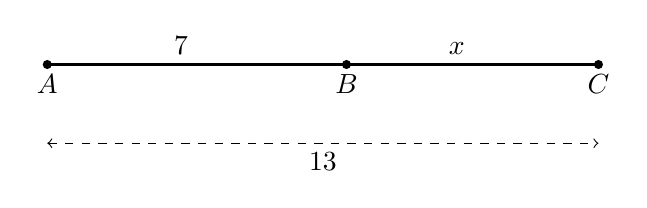
\begin{tikzpicture}
      \draw[fill] (0,0) circle [radius=0.05] node[below]{$A$};
      \draw[thick] (0,0)--(7,0);
      \draw[fill] (3.8,0) circle [radius=0.05] node[below]{$B$};
      \draw[fill] (7,0) circle [radius=0.05] node[below]{$C$};
      \node at (1.7,0) [above]{$7$};
      \node at (5.2,0) [above]{$x$};
      \draw[<->, dashed] (0,-1)--(7,-1);
      \node at (3.5,-1) [below]{$13$};
    \end{tikzpicture}
  \end{center}
  \begin{enumerate}
    \item Circle the equation that most simply represents the situation. \medskip
    \begin{columns}[c]
      \column{0.6\textwidth}
      \qquad \hspace{2cm} $7 + x = 13$
      \column{0.4\textwidth}
      $x = 13 - 7$
    \end{columns}
    \item Find $BC$.
  \end{enumerate} \vspace{2cm}
  Lesson: Vocabulary and notation
  \end{frame}

\section{1.4 Midpoint and bisector \hfill 13 September}
\begin{frame}{Learning Target: I can \emph{bisect} a length}
  {CCSS: HSG.CO.A.1 Know precise geometric definitions  \hfill \alert{1.4 Tuesday 13 Sept}}
  \begin{block}{Do Now: Circle or mark each object in the plane}
    \begin{enumerate} 
      \item The point $H$
      \item The ray $\overrightarrow{JL}$
      \item The name of the plane shown
      \end{enumerate}
    \begin{center}
    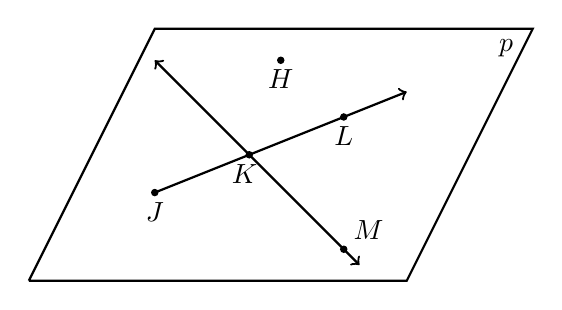
\begin{tikzpicture}[scale=0.8]
      \draw[thick](0,0)--(6,0)--(8,4) node[below left]{$p \ $} --(2,4)--(0,0);
      \draw[->, thick] (2, 1.4)--(6,3);
      \draw[fill] (4, 3.5) circle [radius=0.05] node[below]{$H$};
      \draw[fill] (2, 1.4) circle [radius=0.05] node[below]{$J$};
      \draw[fill] (3.5,2) circle [radius=0.05] node[below]{$K \ $};
      \draw[fill] (5,2.6) circle [radius=0.05] node[below]{$L$};
      \draw[<->, thick] (2,3.5)--(5.25,.25);
      \draw[fill] (5,0.5) circle [radius=0.05] node[above right]{$M \ $};
    \end{tikzpicture}
    \end{center}
    \end{block}
    Lesson: Midpoint, congruence, bisection
  \end{frame}

\section{1.5 Equilateral and isosceles triangles, perimeter \hfill 14 September}
\begin{frame}{Learning Target: I can work with objects having congruent parts}
  {CCSS: HSG.CO.A.1 Know precise geometric definitions  \hfill \alert{1.5 Wednesday 14 Sept}}
    \begin{block}{Do Now: Given $\overline{ST}$ with $S(-2)$ and $T(4)$}
      \begin{center}
      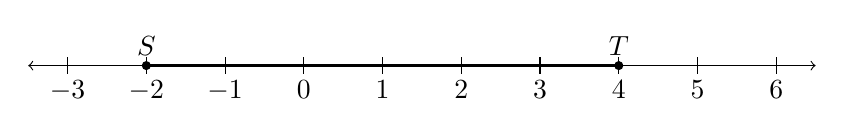
\begin{tikzpicture}
        \draw[<->] (-3.5,0)--(6.5,0);
        \foreach \x in {-3,...,6}
          \draw[shift={(\x,0)}] (0pt,-3pt)--(0pt,3pt) node[below=5pt]{$\x$};
        \draw[fill] (-2,0) circle [radius=0.05] node[above]{$S$};
        \draw[fill] (4,0) circle [radius=0.05] node[above]{$T$};
        \draw[thick] (-2,0)--(4,0);
      \end{tikzpicture}
      \end{center}
    What is the length of the segment $\overline{ST}$? Show your work as an equation.
    \end{block} \vspace{2cm}
    Lesson: Perimeter, congruent line segments in rectangles \& isosceles triangles
  \end{frame}

\section{1.6 Roundtable review \hfill 15 September}
\begin{frame}{Learning Target: I can collaborate in review}
  {CCSS: HSG.CO.A.1 Know precise geometric definitions  \hfill \alert{1.6 Thursday 15 September}}
  Do Now: Given the points $X$ and $Y$, draw $\overrightarrow{YX}$. \par \bigskip
  (careful! which direction does it go?) 
  \vspace{1cm}
  \begin{center}
    \begin{tikzpicture}
    \draw[fill] (1,2) circle [radius=0.05] node[below]{$X$};
    \draw[fill] (5,0) circle [radius=0.05] node[below]{$Y$};
  \end{tikzpicture}
  \end{center} \vspace{1cm}
  Lesson: Roundtable quiz review
\end{frame}

\section{1.7 Unit conversion, Exit note quiz \hfill 16 September}
\begin{frame}{Learning Target: I can change units of length}
  {CCSS: HSG.CO.A.1 Know precise geometric definitions  \hfill \alert{1.7 Friday 16 September}}
  Do Now: Mike is six feet tall. How many inches is that? \par \medskip
  Conversion: 1 foot = 12 inches \par
  \vspace{3cm}
  \alert{Exit note quiz today}
  \end{frame}

\end{document}